\section{Měření}

Prvním zajímavým experimentem bylo měření rychlosti vyhledávání při plné databázi (295 skladeb) v závislosti na délce dotazu. Vstupní melodii jsem postupně zvyšoval od 3 not až na 40 not. Testoval jsem jak oba dva mnou implementované algoritmy (LCS a DTW), tak také pro zajímavost algoritmus fastDTW \cite{fastdtw}, dostupný jako Python package, který by měl DTW implementovat v lineárním čase a paměti.

Z grafu je patrné, že LCS a DTW jsou ovlivňovány délkou dotazu lineárně, což částečně potvrzuje, že oba mají složitost $O(mn)$. DTW je však pomalejší o nějakou konstantu -- průměr této konstanty byl ${6,61}$.

Naopak fastDTW byl ovlivněn délkou dotazu minimálně, což odpovídalo předpokladu, že algoritmus skutečně pracuje v lineárním čase.

\begin{figure}[!ht]
    \caption{Graf závislosti délky vstupní melodie a rychlosti vyhledávání algoritmů}
    \centering
    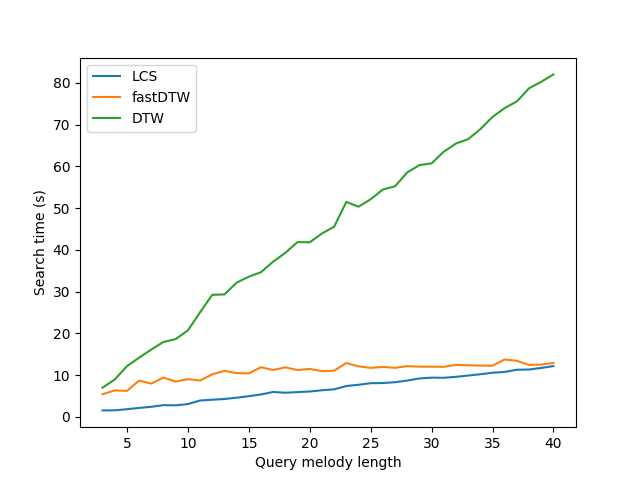
\includegraphics[width=\textwidth]{images/query_len.png}
\end{figure}


V dalším experimentu jsem zkoumal opět na odlišné délce vstupní melodie, jak se vyvíjí průměrná délka největší společné podsekvence ku maximální možné délce společné podsekvence (tedy plná délka vstupní melodie). V podstatě tato hodnota udává, jak moc podobné jsou všechny nejlepší segmenty každé skladby (prozkoumáno vždy všech 295 skladeb v databázi) vstupní melodii.

\begin{figure}[!ht]
    \caption{Graf závislosti délky vstupní melodie a průměrné podobnosti}
    \centering
    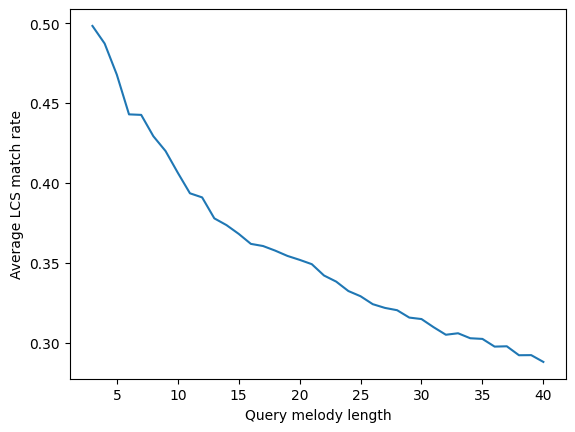
\includegraphics[width=\textwidth]{images/lcs_match_rate.png}
\end{figure}

V grafu je vidět, že při velmi malém vstupu dokážeme najít opravdu hodně velmi podobných segmentů -- průměrná podobnost se pohybuje mezi $45-50 \%$. Při středně velkém vstupu (10--15) však průměrná podobnost rychle klesá, a při velkých vstupech (25--40) klesá pomaleji.

Vývoj této metriky můžeme interpretovat tak, že velmi malé vstupy nejsou přiliš užitečné pro to, abychom v seznamu výsledků našli to, co hledáme -- v seznamu totiž bude mnoho skladeb s vysoce podobnými segmenty. Stačí však zadat o trochu delší vstup a průměrná hodnota podobnosti rychle klesá, a tím pádem seznam výsledků bude trochu čitelnější.
